\documentclass[]{beamer}
%\usepackage[utopia]{mathdesign}
%\usepackage[no-math]{fontspec}
%\setmainfont{Liberation Serif}

\usepackage{minted}
% \usepackage{redhat}
\usepackage{hyperref}
\usepackage{ccicons}
\usepackage{ulem}

\usepackage{tikz}
\usetikzlibrary{arrows,shapes,snakes,automata,backgrounds,petri}

%gets rid of bottom navigation bars
\setbeamertemplate{footline}[frame number]{}

%gets rid of navigation symbols
\setbeamertemplate{navigation symbols}{}

\newcommand{\done}{\textcolor{teal}{\checkmark}}
\newcommand{\pull}[3]{\href{https://github.com/systemd/#1/pulls/#2}{#3 (\##2)}}
\newcommand{\pulldone}[3]{\pull{#1}{#2}{#3} \done}
\newcommand{\commit}[3]{\href{https://github.com/systemd/#1/commit/#2}{#3 (#2)}}
\newcommand{\commitdone}[3]{\commit{#1}{#2}{#3} \done}
\newcommand\pp\pause
%\newcommand\pp{}
\newcommand{\secsec}[1]{\begin{frame}[c]\Huge \textsc #1\end{frame}}

\title{\textsc{mkosi-initrd:\\initrds built from system packages}}
\author{\\
  \includegraphics[height=2em]{images/blue-pacman-192x192.png}\\[1em]
  Zbigniew Jędrzejewski-Szmek\\
  \textit{zbyszek@in.waw.pl}\\[1em]
}
\institute{%
  
\includegraphics[width=0.4\textwidth]{images/Logo-redhat-color-375.png}\\[1em]
  \medskip
  \ccbysa
}
\date{\tiny ASG Berlin 2024, 26.9.2024}

\begin{document}

\setbeamertemplate{itemize items}[square]

\begin{frame}
\titlepage % Print the title page as the first slide
\end{frame}

\secsec{Why?}

\begin{frame}
  \frametitle{Why?}

  Current approach to initrds

%%   \pp
%%   goals:

%%   \begin{itemize}
%%   \item speed → event-driven logic
%%   \item speed → size minimization
%%   \item flexibility, versability, end-user choice
%%   \item local configuration embedded in the initrd
%%   \end{itemize}

%%   \pp
%%   results:

  \pp

  \begin{itemize}
  \item take files from host fs,\\
    \texttt{ldd} to resolve dependencies
  \pp

  \item the packaging layer is duplicated
  \pp

  \item lots of CPU cycles burnt during each kernel update
  \pp

  \quad

  \item at runtime: custom logic (e.g. dracut's initqueue)
  \pp

  \item custom tools (e.g. scripts to bring up LVM, dracut modules)
  \pp

  \item ``custom'' execution environment
  \pp

  \item complexity (in particular when dracut is used with systemd)
  \pp

  \quad

  \item very little sharing of initrd logic between distros
  \end{itemize}
\end{frame}

\begin{frame}
  \frametitle{Why?}

  \pp

  See Wednesday's keynote:\\
  \href{https://cfp.all-systems-go.io/all-systems-go-2024/talk/MRDURE/}
       {``Reproducible and Immutable OS Images\pp{} (with NixOS)''}
  \\\pp

  UKI
  \\\pp
  => combined kernel+initrd (and signed!)
  \\\pp
  => initrd must be built by the vendor/distro
  \\\pp
  => no local modifications
  \\\pp
  => a system designed for local modifications is not useful
  \\\quad
  \\\pp

  if we are building in a package builder, let's build directly from distro packages\\
    (we \textit{could} build from files in the fs, but why?)
\end{frame}

\begin{frame}
  \frametitle{mkosi}
  \framesubtitle{``\textbf{M}a\textbf{K}e \textbf{O}perating \textbf{S}ystem \textbf{I}mage''}

  Build OS images from distro packages (debs, rpms, …)
  \\

  \pp
  Uses \texttt{apt}, \texttt{dnf}, \texttt{dnf5}, \texttt{zypper}, \texttt{pacman}
  \\

  \pp
  Now uses \texttt{systemd-repart} → fully unprivileged operation
  \\

  \pp
  Profiles and [Match] sections → flexibility
  \\
  
  \small
  \pp
  Sam Leonard,
  \href{https://cfp.all-systems-go.io/all-systems-go-2024/talk/9JKWCT/}
       {``Improving systemd’s integration testing infrastructure''}
  \\\quad
  Jelle van der Waa,
  \href{https://cfp.all-systems-go.io/all-systems-go-2024/talk/QFUGLT/}
      {``Creating Arch Linux images using mkosi''}

  \pp

  Daan De Meyer,
  \href{https://0pointer.net/blog/a-re-introduction-to-mkosi-a-tool-for-generating-os-images.html}
       {``A re-introduction to mkosi --- A Tool for Generating OS Images''}\\
  \href{https://media.ccc.de/v/all-systems-go-2023-190-mkosi-building-bespoke-operating-system-images}
       {``mkosi: Building Bespoke Operating System Images''} @ ASG 2023\\
  \href{https://media.ccc.de/v/all-systems-go-2023-191-systemd-repart-building-discoverable-disk-images}
       {``systemd-repart: Building Discoverable Disk Images''} @ ASG 2023\\

  %% see Vitaly Kuzentsov's \\
  %% \href{https://devconfcz2023.sched.com/event/1MYg7/confidential-vms-in-the-cloud}
  %%      {\textsc{``Confidential VMs in the cloud''}}
  %% \\\quad
  %% Christophe de Dinechin's \\
  %% \href{https://devconfcz2023.sched.com/event/1MYgS/confidential-computing-from-host-to-workload}
  %%      {\textsc{``Confidential Computing, from host to workload''}}
  %% \\\quad
\end{frame}

\begin{frame}
  \frametitle{Why distro packages?}

  \begin{itemize}
    \pp
  \item \textbf{less} things
    \pp
  \item we use package dependency resolution mechanism
    \pp
  \item we let rpm/deb/pacman handle 98\% of the installation
    \pp
  \item we don't pull files from the host
    \pp
  \item images can be reproducible
    \pp
  \item images are the same for everyone
    \pp
  \item images signed by vendor
    \pp
  \item systemd does the heavy lifting in the initrd
%%     \pp
%%   \item bash helpers → compiled programs
%%     \pp
%%   \item developers don't need to learn another system\\
%%     (initrd is like a normal system,\\
%%     \phantom( just on an fs not backed by a disk)
%%     \pp
%%   \item clear ownership of bugs
%%     \pp
%%   \item initrd infrastructure can be shared between distros
  \end{itemize}
\end{frame}

%% \begin{frame}
%%   \frametitle{Drawbacks}

%%   We get fully functional initrds, but…
%%   \\\quad
%%   \pp

%%   The initrds are \textbf{bigger}.\\
%%   \pp
%%   Most of the difference is caused by kernel modules
%%   \\\quad

%%   \pp
%%   Only some subset of installations is supported
%% \end{frame}

%% \begin{frame}
%%   1st extension mechanism: credentials
%% \end{frame}

\secsec{Nitty-gritty}

\begin{frame}[fragile]
  \frametitle{How the idea of mkosi-initrd has evolved}

  \pp
  0. PoC, config for mkosi, works on a Thinkpad
  \\

  \pp
  1. Goal: conquer the world — iscsi, fcoe, nfs, raid, kdump, networking!!
\end{frame}

\begin{frame}[fragile]
  \frametitle{How the idea of mkosi-initrd has evolved}
  \framesubtitle{…ctd., example}

  \pp
  iscsi:
  iscsi-initiator-utils
  → 4 binaries, 6 service files
  \\

  \pp
  /usr/lib/dracut/modules.d/95iscsi/cleanup-iscsi.sh
  /usr/lib/dracut/modules.d/95iscsi/iscsiroot.sh
  /usr/lib/dracut/modules.d/95iscsi/module-setup.sh
  /usr/lib/dracut/modules.d/95iscsi/mount-lun.sh
  /usr/lib/dracut/modules.d/95iscsi/parse-iscsiroot.sh\\
  → approx. 1000 lines of bash code generating bash code to wrap the binaries
  \pp

  \begin{minted}{ini}
# iscsi-init.service
[Service]
ExecStart=/usr/bin/sh -c
  'echo "InitiatorName=`/usr/sbin/iscsi-iname`"
  > /etc/iscsi/initiatorname.iscsi'
  \end{minted}

  \pp
  \begin{minted}{console}
$ dracut --list-modules | wc -l
119
\end{minted}
\end{frame}

\begin{frame}
  \frametitle{How the idea of mkosi-initrd has evolved}
  \framesubtitle{…ctd.}

  \pp
  2. Updated goal: make ``new initrds'' work correctly for simple cases, build the infrastructure
  \\

  \pp
  3. Allow easy local use, preprare for centralized builds
\end{frame}

\begin{frame}[fragile]
  \frametitle{Initrds and … exitrds}

  \pp
  In the dracut approach, the initrd saves a compressed subset of itself in memory to unpack and execute shutdown.
  \\

  \pp
  Why waste memory? Why execute old code?
  \\

  \pp
  ``exitrd'' — code to execute at shutdown to clean up the root file system
  \\

  \pp
  systemd has this covered: \texttt{systemd-shutdown}\\
  \texttt{systemd-standalone-shutdown.rpm}
\end{frame}

\secsec{Next steps}

\begin{frame}
  \frametitle{Consequences of centralized builds}
  \framesubtitle{If we use pre-built images, how to deliver differentiated code?}
  \pp

  \begin{enumerate}
    \addtocounter{enumi}{-1}
  \item initrd variants
  \item ``addons'' → checked via SecureBoot db / shim
  \item systemd-sysexts → checked via kernel keyring
  \item systemd-confexts
  \item credentials → encrypted via TPM|local key
  \end{enumerate}

%%   \vfill

%%   \pp
%%   Building of sysexts depends build reproducibility of the initrd
\end{frame}

\begin{frame}
  \frametitle{steps towards world domination}

  \pp
  mkosi-initrd is now part of mkosi,\\
  installed as \texttt{/usr/lib/kernel/install.d/50-mkosi.install}
  \\

  \pp
  support for openssl ``signing engines'', sbsign, pesign\\
  \pp
  (open pull request for) offline signing
  \\
  
  \pp
  mkosi can build sysexts, but it's still PoC
  \\
  
  \pp
  mkosi / mkosi-initrd can detect the CPU vendor and build µcode initrd
  => \texttt{.ucode} section
\end{frame}

\begin{frame}
  \frametitle{The ``big initrd'' problem}

  \pp
  the problem is general: drivers, firmware, composefs, …
  \\

  \pp
  copying is fast, decompression is slow => avoid decompression
  \\

  \pp
  the kernel may allow zero-copy donation of fs image
\end{frame}

%% \begin{frame}
%%   \frametitle{Credentials}
%%   \pp

%%   A generic mechanism:\\\\
%%   data → \\
%%   file (\texttt{/etc/credstore/data}) | other storage → \\
%%   service has \texttt{LoadCredential=data} → \\
%%   manager passes the credential → \\
%%   service sees \texttt{\$CREDENTIALS\_DIRECTORY/data}

%%   \pp
%%   \quad

%%   file | pipe | \\
%%   qemu \texttt{SMBIOS} | \texttt{fw\_cfg} | \\
%%   kernel command-line | \\
%%   boot loader | \\
%%   inherited credential
%% \end{frame}

%% \begin{frame}[fragile]
%%   \frametitle{Credential encryption}
%%   \framesubtitle{(with machine keys)}

%%   \pp
%%   data → \\
%%   \textbf{\texttt{systemd-creds encrypt}} → \\
%%   file | other storage → \\
%%   \texttt{LoadCredential\textbf{Encrypted}=} → \\
%%   \textbf{manager decrypts} → \\
%%   service sees \texttt{\$CREDENTIALS\_DIRECTORY/data}

%%   \pp
%%   \quad

%%   Encryption with:\\
%%   - \texttt{/var/lib/systemd/credential.secret}
%%   \\
%%   - TPM2
%%   \\
%%   - both

%%   \vfill

%%   \small
%%   \url{https://systemd.io/CREDENTIALS}
%% \end{frame}

%% \begin{frame}
%%   2nd extension mechanism: confexts
%% \end{frame}

%% \begin{frame}
%%   \frametitle{confexts (and sysexts)}
%%   \framesubtitle{``Configuration Extensions''\\
%%                  ``System Extensions''}

%%   sysext — partial system image that is \texttt{overlayfs}ed on the host system:
%%   \textcolor{blue}{\texttt{/usr}} and \textcolor{blue}{\texttt{/opt}}
%%   \\\quad\pp

%%   confext — partial system image that is \texttt{overlayfs}ed on the host system:
%%   \textcolor{blue}{\texttt{/etc}}

%% %%   \vfill

%% %%   \pp
%% %%   Building of sysexts depends build reproducibility of the initrd
%% \end{frame}

%% \begin{frame}
%%   \frametitle{Discoverable Disk Images}

%%   \href{https://uapi-group.org/specifications/specs/discoverable_partitions_specification/}{The Discoverable Partitions Specification}\\
%%   (recognition of file system role by part-type UUID)
%%   \\\quad\pp

%%   \texttt{systemd-dissect <image>}
%%   \\\quad\pp

%%   \texttt{systemd-dissect --mount <image> <path>}
%%   \\\quad\pp

%%   \texttt{systemd-dissect --mtree <image>}
%% \end{frame}

%% \begin{frame}
%%   \frametitle{systemd-dissect <image>}

%%   \hspace*{-2em}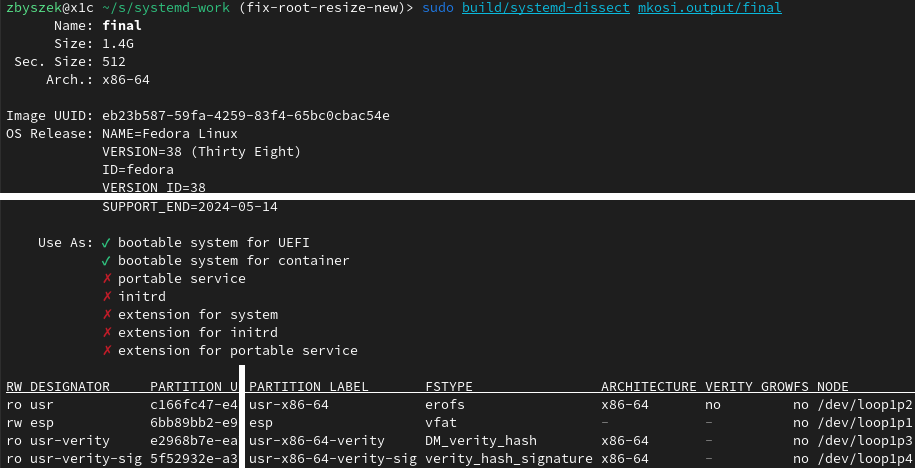
\includegraphics[width=1.15\textwidth]{images/systemd-dissect.png}
%% \end{frame}

%% \begin{frame}
%%   \frametitle{What are DDIs good for?}

%%   operating system image → hardware or VM or container
%%   \\\quad

%%   portable service
%%   \\\quad

%%   % initrd?

%%   system extension
%%   \\\quad

%%   initrd extension
%%   \\\quad

%%   portable service extension
%% \end{frame}

%% \begin{frame}
%%   \frametitle{What are System Extensions good for?}

%%   \pp
%%   \textcolor{teal}{Reminder:}{ }\begin{minipage}[t]{0.8\linewidth}
%%     the initrd is a compressed cpio archive

%%     \quad

%%     a sysext is a GPT image with
%%     three partitions:\\
%%     the filesystem (e.g.\ compressed squashfs),
%%     dm-verity for the filesystem,
%%     signature for the verity data
%%   \end{minipage}

%%   \quad

%%   \begin{itemize}
%%     \pp
%%   \item a network configuration daemon + sshd

%%     \pp
%%   \item nfs / RAIDs / clevis / network storage

%%     \pp
%%   \item the full graphical stack\pp: a11y! \pp i18n!

%%     \pp
%%   \item the full sound stack\pp: a11y!

%%     \pp
%%   \item hardware enablement, incl. bluetooth

%%     \pp
%%   \item (suggestions welcome)
%%   \end{itemize}
%% \end{frame}

%% \begin{frame}
%%   \frametitle{What does the kernel say?}

%%   \pp
%%   (the short answer: it doesn't care)

%%   \hfill

%%   \pp
%%   the long answer:
%%   the initrd is just an in-memory file system\\
%%   \texttt{/init} is started instead of \texttt{/sbin/init}
%% \end{frame}

%% \begin{frame}
%%   \frametitle{New goals}

%%   \begin{itemize}
%%     \pp
%%   \item reuse distro packaging
%%     \pp
%%   \item use systemd in the initrd
%%     \pp
%%   \item use normal services
%%     \pp
%%   \item standard userspace environment
%%     \pp
%%   \item reasonable size
%%     \pp

%%   \quad

%%   \item build reproducible initrd images
%%     \pp
%%   \item build initrd images on vendor systems
%%     \pp
%%   \item sign the kernel + initrd
%%     \pp
%%   \item build a set of System Extension images for the initrd
%%     \pp
%%   \item sign those too
%%     \pp

%%   \quad

%%   \item maintainers of user-space packages handle ``initrd bugs''
%%   \end{itemize}
%% \end{frame}

%% \begin{frame}
%%   3rd extension mechanism: ``addons''
%% \end{frame}

%% \begin{frame}
%%   \frametitle{``Addons''}

%%   UKI-like binaries with kernel parameters
%% \end{frame}


\begin{frame}
  \frametitle{Summary: short list of tools \& concepts}

  \pp
  mkosi \\
  mkosi-initrd | 50-mkosi.install \\
  ukify | 60-ukify.install \\
  kernel-install \\
  systemd-measure \\
  pesign | sbsign \\
  addons | sysexts | confexts | credentials \\
  sd-stub \\
  reproducible builds \\
  UKIs | multi-profile UKIs | incremental builds | offline signing\\
  cpio | squashfs | EROFS | zero-copy unpacking \\
  immutable \& signed initrd

\end{frame}

\begin{frame}[fragile]
  \frametitle{Links}

  \url{https://github.com/systemd/mkosi}

  \url{https://www.freedesktop.org/software/systemd/man/systemd-sysext.html}

  {
    \small
    \url{https://gitlab.com/cryptsetup/cryptsetup/-/wikis/DMVerity}\\
    \color{gray}{\url{https://www.kernel.org/doc/html/latest/admin-guide/device-mapper/verity.html}}
    }

  \url{https://www.kernel.org/doc/html/latest/filesystems/overlayfs.html}

  \quad

  These slides:
  \url{https://github.com/keszybz/mkosi-initrd-talk/raw/main/asg2024-mkosi-initrd.pdf}

  \quad
  \pp

  \hfill \textcolor{red}{QUESTIONS?} \textcolor{green}{\bf /} \textcolor{red}{EOF} \hfill{}
\end{frame}

\begin{frame}
\end{frame}

\begin{frame}
  \frametitle{Objections?}

% If you have some experience in this area,
% and you think that this just infeasible/inefficient/unreasonable, consider that:

  \begin{itemize}
    \pp
    \item
      systemd was already used in the initrd
    \pp
    \item
      the first thing systemd does is to set up the environment
    \pp
    \item
      having tools that support running in a custom environment is hence not useful
    \pp
    \item
      after removing custom logic we don't need to add anything back
    \pp
    \item
      the ecosystem is moving away from scripts towards compiled daemons
    \pp
    \item
      most of the code is in shared libraries, which are installed in full because of link dependencies
    \pp
    \item
      error handling, timeouts, retries, localized messages, event-driven logic, netlink,
      D-bus, all are much easier with ``real'' code
  \end{itemize}
\end{frame}

\end{document}
